%%%%%%%%%%%%%%%%%%%%%%%%%%%%%%%%%%%%%%%%%
% Beamer Presentation
% LaTeX Template
% Version 1.0 (10/11/12)
%
% This template has been downloaded from:
% http://www.LaTeXTemplates.com
%
% License:
% CC BY-NC-SA 3.0 (http://creativecommons.org/licenses/by-nc-sa/3.0/)
%
%%%%%%%%%%%%%%%%%%%%%%%%%%%%%%%%%%%%%%%%%

%----------------------------------------------------------------------------------------
%	PACKAGES AND THEMES
%----------------------------------------------------------------------------------------

\documentclass{beamer}

\mode<presentation> {

% The Beamer class comes with a number of default slide themes
% which change the colors and layouts of slides. Below this is a list
% of all the themes, uncomment each in turn to see what they look like.

%\usetheme{default}
%\usetheme{AnnArbor}
%\usetheme{Antibes}
%\usetheme{Bergen}
%\usetheme{Berkeley}
%\usetheme{Berlin}
%\usetheme{Boadilla}
%\usetheme{CambridgeUS}
%\usetheme{Copenhagen}
%\usetheme{Darmstadt}
%\usetheme{Dresden}
%\usetheme{Frankfurt}
%\usetheme{Goettingen}
%\usetheme{Hannover}
%\usetheme{Ilmenau}
%\usetheme{JuanLesPins}
%\usetheme{Luebeck}
\usetheme{Madrid}
%\usetheme{Malmoe}
%\usetheme{Marburg}
%\usetheme{Montpellier}
%\usetheme{PaloAlto}
%\usetheme{Pittsburgh}
%\usetheme{Rochester}
%\usetheme{Singapore}
%\usetheme{Szeged}
%\usetheme{Warsaw}

% As well as themes, the Beamer class has a number of color themes
% for any slide theme. Uncomment each of these in turn to see how it
% changes the colors of your current slide theme.

%\usecolortheme{albatross}
%\usecolortheme{beaver}
%\usecolortheme{beetle}
%\usecolortheme{crane}
%\usecolortheme{dolphin}
%\usecolortheme{dove}
%\usecolortheme{fly}
%\usecolortheme{lily}
%\usecolortheme{orchid}
%\usecolortheme{rose}
%\usecolortheme{seagull}
%\usecolortheme{seahorse}
%\usecolortheme{whale}
%\usecolortheme{wolverine}

%\setbeamertemplate{footline} % To remove the footer line in all slides uncomment this line
%\setbeamertemplate{footline}[page number] % To replace the footer line in all slides with a simple slide count uncomment this line

%\setbeamertemplate{navigation symbols}{} % To remove the navigation symbols from the bottom of all slides uncomment this line
}

\usepackage{graphicx} % Allows including images
\usepackage{booktabs} % Allows the use of \toprule, \midrule and \bottomrule in tables
\usepackage{multirow}
\usepackage{adjustbox}
\usepackage{array}
\usepackage{tikz}
\usepackage{soul}
\usetikzlibrary{shapes.geometric, arrows, positioning, fit}
\usepackage[latin1]{inputenc}
\newcommand{\xmark}{\textcolor{red}{\text{\sffamily X}}}
\newcommand{\cmark}{\textcolor{green}{\checkmark}}
\newcommand{\tr}{\text{tr}}
\newcommand{\E}{\textbf{E}}
\newcommand{\diag}{\text{diag}}
\newcommand{\argmax}{\text{argmax}}
\newcommand{\argmin}{\text{argmin}}
\newcommand{\Cov}{\text{Cov}}
\newcommand{\Var}{\text{Var}}
\newcommand{\Vol}{\text{Vol}}
\newcommand{\bx}{\boldsymbol{x}}
\newcommand{\by}{\boldsymbol{y}}
\newcommand{\bX}{\boldsymbol{X}}
\newcommand{\bY}{\boldsymbol{Y}}
\sethlcolor{gray}
\makeatletter
\newcommand\SoulColor{%
  \let\set@color\beamerorig@set@color
  \let\reset@color\beamerorig@reset@color}
\makeatother
\definecolor{color1}{RGB}{128,13,13}
\definecolor{color2}{RGB}{70,128,13}
\definecolor{color3}{RGB}{13,128,128}
\definecolor{color4}{RGB}{70,13,128}

%tikz stufff


%----------------------------------------------------------------------------------------
%	TITLE PAGE
%----------------------------------------------------------------------------------------

%"Estimating mutual information for high-dimensional sparse relationships"

%Abstract: Mutual information is a versatile measure of the strength of
%nonlinear dependence between two random variables or vectors.
%However, estimating mutual information in high dimensions requires
%prohibitively large numbers of observations, which limits its use in
%many applications of interest.  We propose a new method for estimating
%mutual information in when the assumption of sparsity can be
%justified--i.e., in situations where there exists a low-dimensional
%structure hidden within the high-dimensional data.  Our method builds
%a bridge between modern statistical and machine learning models for
%"learning from sparsity" and the classical problem of estimating
%mutual information, exploiting the assumption of sparsity to achieve
%effective estimation even with relatively few observations.  We
%demonstrate the utility of our approach in simulations, and a
%gene-expression time series data set.

\title[Mutual information]{Estimating mutual information for high-dimensional sparse relationships}

\author{Charles Zheng} % Your name
\institute[Stanford] % Your institution as it will appear on the bottom of every slide, may be shorthand to save space
{Stanford University}
\date{\today} % Date, can be changed to a custom date

\begin{document}

\begin{frame}
\titlepage % Print the title page as the first slide
(Joint work with Yuval Benjamini, Hebrew University.)
\end{frame}


\section{Introduction}

\begin{frame}
\frametitle{Introduction}
\begin{center}
%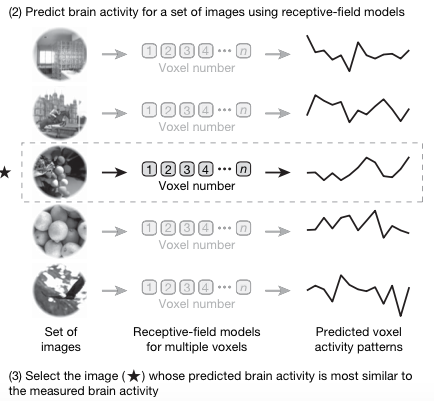
\includegraphics[scale = 0.3, clip=true, trim = 0 0in 0 0]{kay01.png}
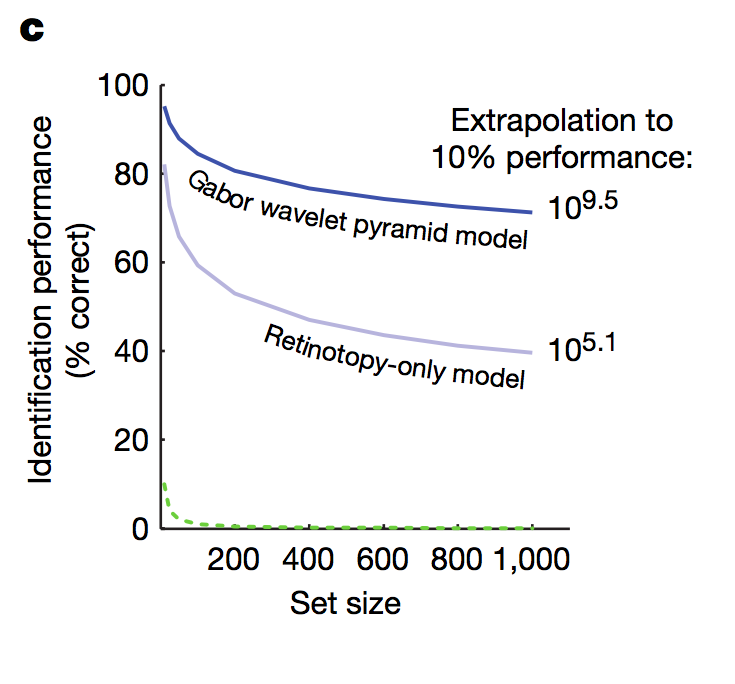
\includegraphics[scale = 0.2, clip=true, trim = 0 0in 0 0]{kay_extrapolation.png}
\end{center}
\begin{itemize}
\item Much of my work has been inspired by use of machine learning in encoding/decoding models in fMRI (Kay et al. 2008, Nishimoto et al. 2011)\pause
\item E.g.: Extrapolating classification accuracy curves (Z., Achanta, and Benjamini 2016)
\end{itemize}
\end{frame}

\begin{frame}
\frametitle{This talk}
\begin{columns}
\begin{column}{0.25\textwidth}
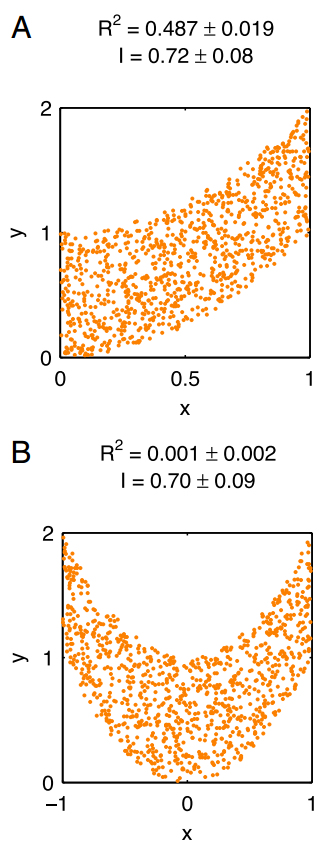
\includegraphics[scale = 0.27]{kinney3.png}
\end{column}
\begin{column}{0.75\textwidth}
Mutual information $I(\vec{X}; \vec{Y})$
\begin{itemize}
\item measures dependence between two random vectors, $\vec{X}$ and $\vec{Y}$ \pause
\item applies to nonlinear and multidimensional relationships (unlike correlation) \pause
\item is \emph{difficult to estimate} in high dimensions \pause
\end{itemize}
We combine \emph{machine learning} (sparse estimation) with \emph{information theory} to obtain better estimates of $I(\vec{X}; \vec{Y})$
\begin{center}
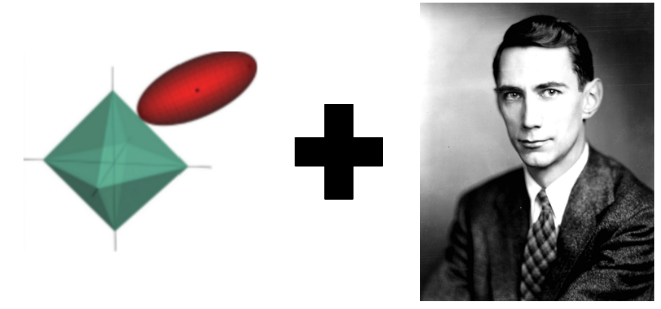
\includegraphics[scale = 0.23]{ml_shann.png}
\end{center}
\end{column}
\end{columns}
\end{frame}

\begin{frame}
\frametitle{Mutual information $I(X; Y)$}
\begin{center}
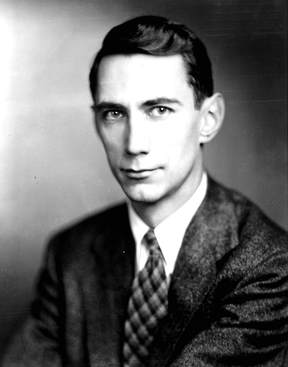
\includegraphics[scale = 0.23]{shannon_claude.png}
\hspace{0.2in}
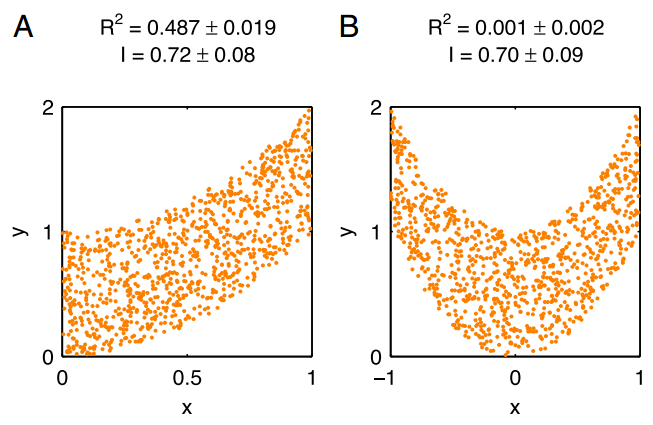
\includegraphics[scale = 0.2]{kinney2.png}
\end{center}
Introduced in Shannon's 1948 paper, ``A mathematical theory of communication''
\[
I(X; Y) = \int \log \left(\frac{p(x, y)}{p(x)p(y)}\right) p(x, y) dx dy
\]
%\begin{itemize}
%\item 
%\item Mutual information measures nonlinear dependence between random variables% $X$ and $Y$
%\end{itemize}

\vspace{0.2in}
\tiny{Image credit Kinney et al. 2014.}
\end{frame}


\begin{frame}
\frametitle{Applications of $I(X; Y)$}
Mutual information has since been applied to many areas outside of information theory\pause
\begin{center}
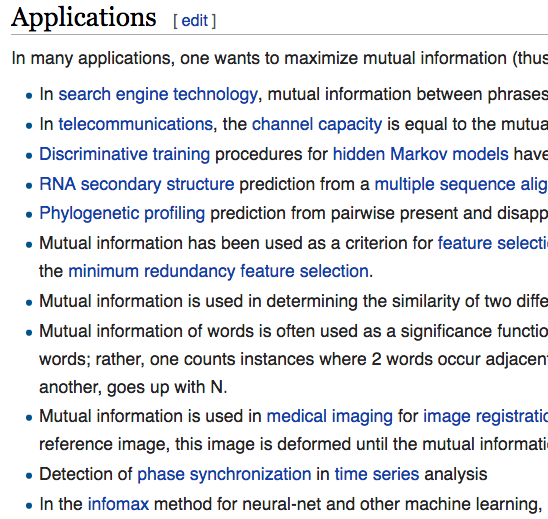
\includegraphics[scale = 0.3]{wiki_apps.png}
\end{center}
Engineering, biology, computer science, physics, medicine
\end{frame}



\begin{frame}
\frametitle{Comparing $I(X; Y)$ with Pearson correlation}
\begin{center}
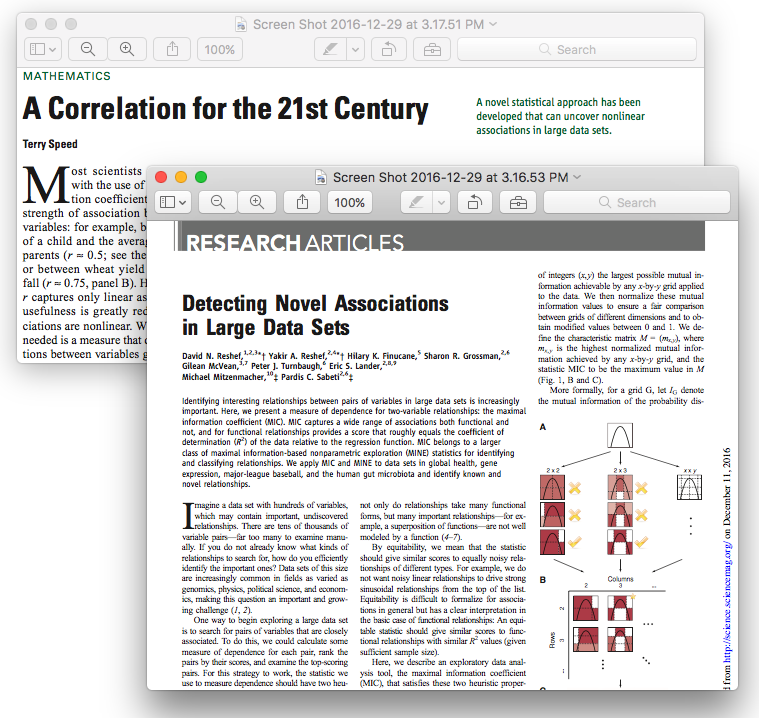
\includegraphics[scale = 0.2]{speed_reshef.png}
\end{center}
\begin{itemize}
\item In many applications scientists are interested in \emph{dependence}, not \emph{correlation} (Reshef et al. 2011, Speed 2011). \pause
\item Only mutual information (and derived quantities) measures dependence directly.
\end{itemize}
\end{frame}

%\begin{frame}
%\frametitle{Mutual information (Shannon 1948)}
%\begin{center}
%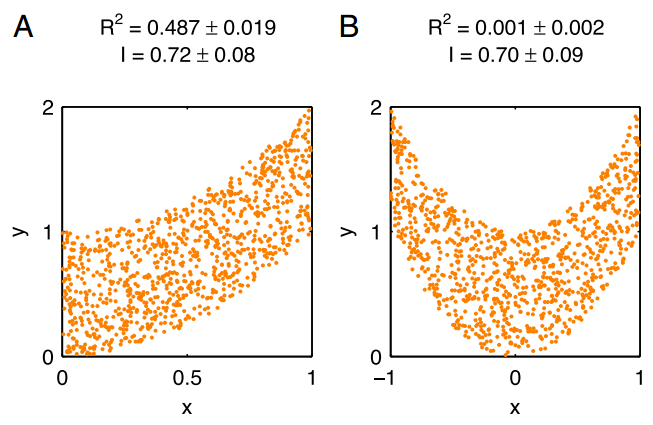
\includegraphics[scale = 0.2]{kinney2.png}
%\end{center}
%\begin{itemize}
%\item $I(X;Y) \geq 0$.\pause
%\item $I(X; Y) = $0 if $X \perp Y$ \pause
%\item Symmetry: $I(X;Y) = I(Y; X)$.\pause 
%\end{itemize}
%\emph{(all of these are also properties of Pearson correlation)}
%\end{frame}

%\begin{frame}
%\frametitle{Mutual information (Shannon 1948)}
%\begin{center}
%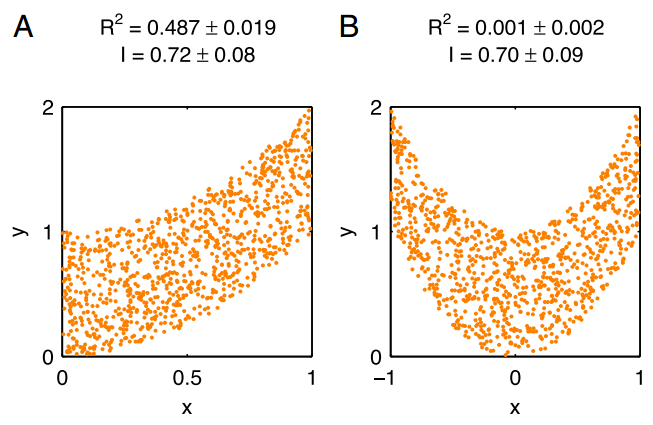
\includegraphics[scale = 0.2]{kinney2.png}
%\end{center}
%\begin{itemize}
%\item Data-processing inequality:
%\begin{itemize}
%\item Transforming $X$ or $Y$ generally \emph{decreases} the information (and can never increase it) \pause
%\item But if the transformation is bijective, the information stays the same (\emph{invariance} under bijections)\pause
%\end{itemize}
%Pearson correlation is invariant only under \emph{linear} bijections--and can otherwise increase under transformations.
%\[I(X; Y) \geq I(\phi(X); \psi(Y))\]
%equality for $\phi$, $\psi$ bijections
%\item Additivity.  If $(X_1,Y_1) \perp (X_2, Y_2)$, then
%\[
%I((X_1, X_2); (Y_1, Y2)) = I(X_1; Y_1) + I(X_2; Y_2).
%\]
%\item Relation to KL divergence
%\[\mathbb{D}(p(x, y)||p(x)p(y)) = I(X; Y).\]
%\end{itemize}
%\end{frame}


\begin{frame}
\frametitle{Problems with mutual information}
\begin{itemize}
\item Hard to interpret (compared to $R^2$) \pause
\begin{itemize}
\item Define the ``informational correlation'' (Linfoot 1957)
\[
\text{Cor}_{Info}(X, Y) = \sqrt{1-e^{-2I(X; Y)}}
\]
\pause
\item Then $\text{Cor}_{Info}(X, Y) \in [0,1]$.
\item For $(X, Y)$ bivariate normal,
\[
|\text{Cor}_{Pearson}(X, Y)| = \text{Cor}_{Info}(X, Y)
\]
\pause
\end{itemize}
\item Hard to estimate (compared to $R^2$)
\end{itemize}
\end{frame}

%\begin{frame}
%\frametitle{Comparing $I(X; Y)$ with Pearson correlation}
%\begin{columns}
%\begin{column}{0.5\textwidth}
%Pearson $R^2$
%\begin{itemize}
%\item[+] Easy to interpret \\(0 = uncorrelated,\\ 1 = perfect correlation)\pause
%\item[+] Straightforwardly estimated
%\item[-] Only applies to univariate $X$, $Y$\pause
%\item[-] Only captures linear associations\pause
%\end{itemize}
%\end{column}
%\begin{column}{0.5\textwidth}
%Mutual information
%\begin{itemize}
%\item[+] Captures nonlinear associations \pause
%\item[+] Extends to arbitrarily many dimensions \pause
%\item[+] Nonlinear invariance \pause
%\item[-] Less easy to interpret? \pause
%\item[-] Harder to estimate from data!
%\end{itemize}
%\end{column}
%\end{columns}
%\end{frame}

%\begin{frame}
%\frametitle{Can we make $I(X; Y)$ easier to interpret?}
%\begin{itemize}
%\item If $(X, Y)$ have a bivariate normal distribution with correlation $\rho$, then
%\[
%I(X; Y) = \frac{-1}{2}\ln(1 - \rho^2)
%\] \pause
%\item Define the ``informational correlation'' (Linfoot 1957)
%\[
%\text{Cor}_{Info}(X, Y) = \sqrt{1-e^{-2I(X; Y)}}
%\]\pause
%\item Then $\text{Cor}_{Info}(X, Y) \in [0,1]$.
%\item For $(X, Y)$ bivariate normal,
%\[
%\text{Cor}_{Pearson}(X, Y)| = \text{Cor}_{Info}(X, Y)
%\]
%\end{itemize}
%\pause 
%\end{frame}

%\begin{frame}
%\frametitle{Difficulty of estimating $I(X; Y)$}
%Example with $\text{Cor}_{Pearson}(X, Y) = \text{Cor}_{Info}(X, Y) = 0.44$.
%\begin{center}
%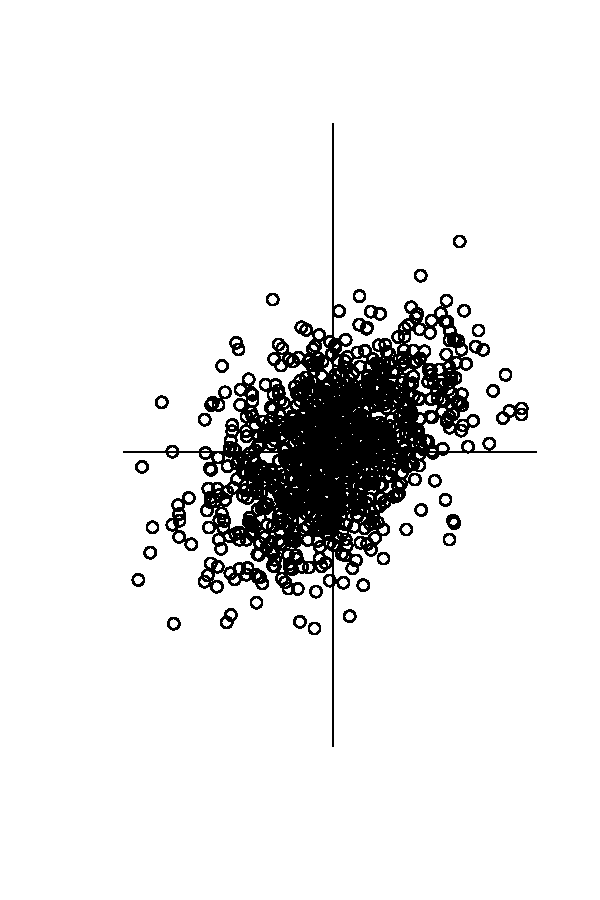
\includegraphics[scale = 0.2, clip=true, trim=0 -2in 0 0]{../info_theory_sims/cor_2.pdf}
%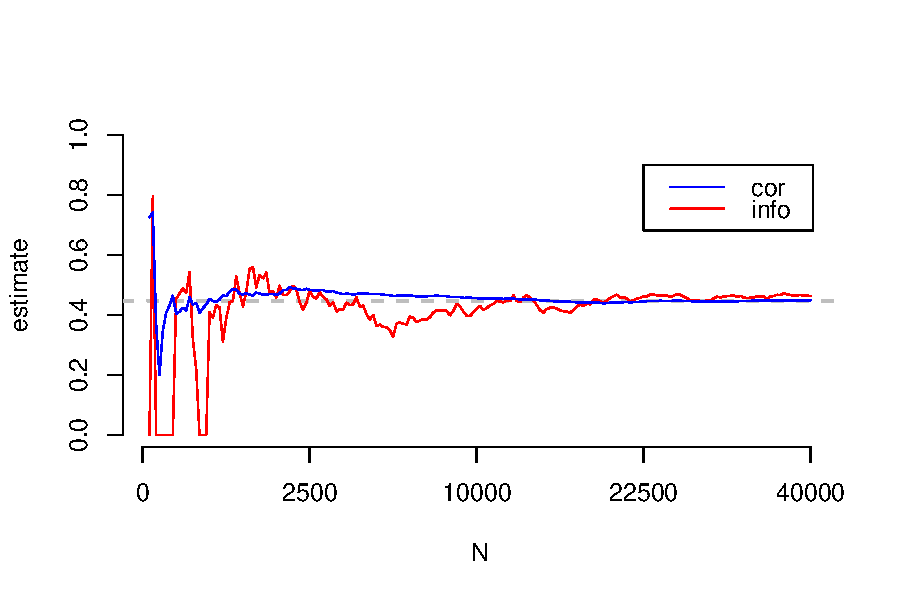
\includegraphics[scale = 0.5]{../info_theory_sims/cor_info2.pdf}
%\end{center}
%\end{frame}


%\begin{frame}
%\frametitle{Difficulty of estimating $I(X; Y)$}
%Example with $\text{Cor}_{Pearson}(X, Y) = \text{Cor}_{Info}(X, Y) = 0.2$.
%\begin{center}
%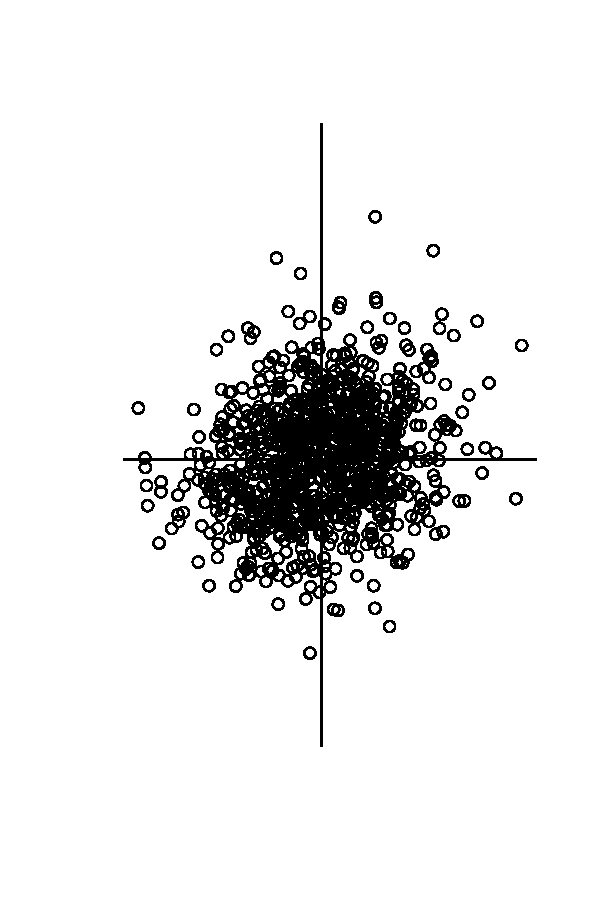
\includegraphics[scale = 0.2, clip=true, trim=0 -2in 0 0]{../info_theory_sims/cor_1.pdf}
%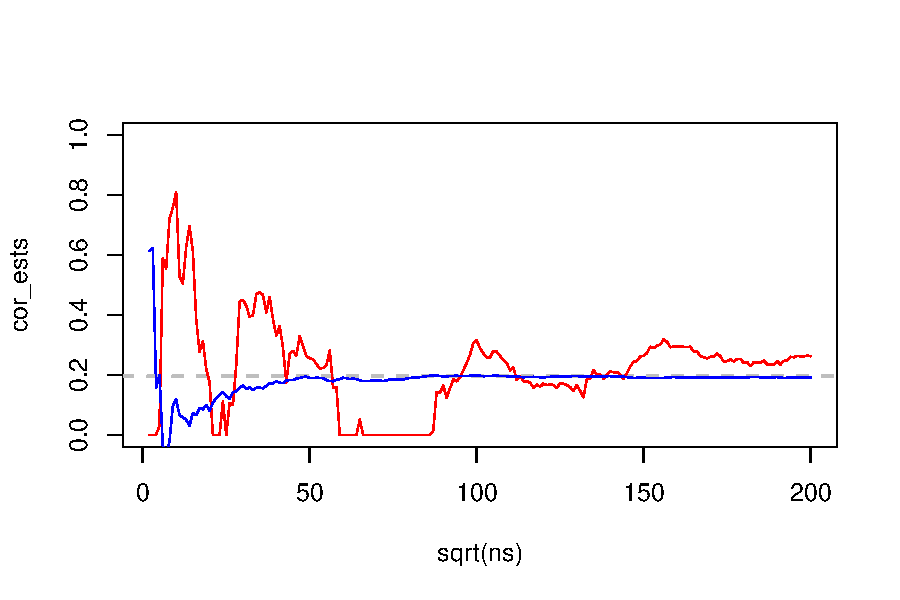
\includegraphics[scale = 0.5]{../info_theory_sims/cor_info1.pdf}
%\end{center}
%\end{frame}

\begin{frame}
\frametitle{How to estimate $I(X; Y)$}
Suppose we observe pairs $(X_i,Y_i)_{i=1}^n$ iid from density $p(x, y)$
\begin{itemize}
\item Definition of mutual information:
\[
I(X; Y) = \int \log \left(\frac{p(x, y)}{p(x)p(y)}\right) p(x, y) dx dy
\]\pause
\item Kernel density estimate approaches estimate $p(x,y)$ (Beirlant et al. 2001, Ivanov and Rozhkova 1981)
\item Nearest neighbor estimators rely on distance-based computations (Mnatsakanov et al. 2008, Goria et al. 2005, Singh et. al. 2003)
\end{itemize}
\end{frame}

\begin{frame}
\frametitle{How to estimate $I(X; Y)$}
Suppose we observe pairs $(X_i,Y_i)_{i=1}^n$ iid from density $p(x, y)$
\begin{itemize}
\item \textbf{Plug-in estimate}:
\[
\hat{I}(X; Y) = \int \log \left(\frac{\hat{p}(x, y)}{\hat{p}(x)\hat{p}(y)}\right) \hat{p}(x, y) dx dy
\]
\item Kernel density estimate approaches estimate $p(x,y)$ (Beirlant et al. 2001, Ivanov and Rozhkova 1981)
\item Nearest neighbor estimators rely on distance-based computations (Mnatsakanov et al. 2008, Goria et al. 2005, Singh et. al. 2003)
\end{itemize}
\end{frame}


\begin{frame}
\frametitle{Problems in high dimensions}
\begin{itemize}
\item Density estimation is known to have \emph{exponential complexity} with respect to dimensionality.
\begin{itemize}
\item E.g. to get the same precision, you need 10 observations for univariate $X, Y$ but 1000 for trivariate $\vec{X}, \vec{Y}$. \pause
\end{itemize}
\item Many applications with high-dimensional $X$, $Y$.
\begin{itemize}
\item Gene expression time series
\item Functional magnetic resonance imaging \pause
\end{itemize}
\item One approach is to assume joint multivariate normality of $X$, $Y$, but this reduces mutual information to a linear statistic. \pause
\item Other approaches: binning (Bialek et al. 1991, Paninski 2003), confusion matrix of a classifier (Treves 1997, Quiroga et al. 2009)
\end{itemize}
\end{frame}


\begin{frame}
\frametitle{New idea: Use sparsity!}
\begin{center}
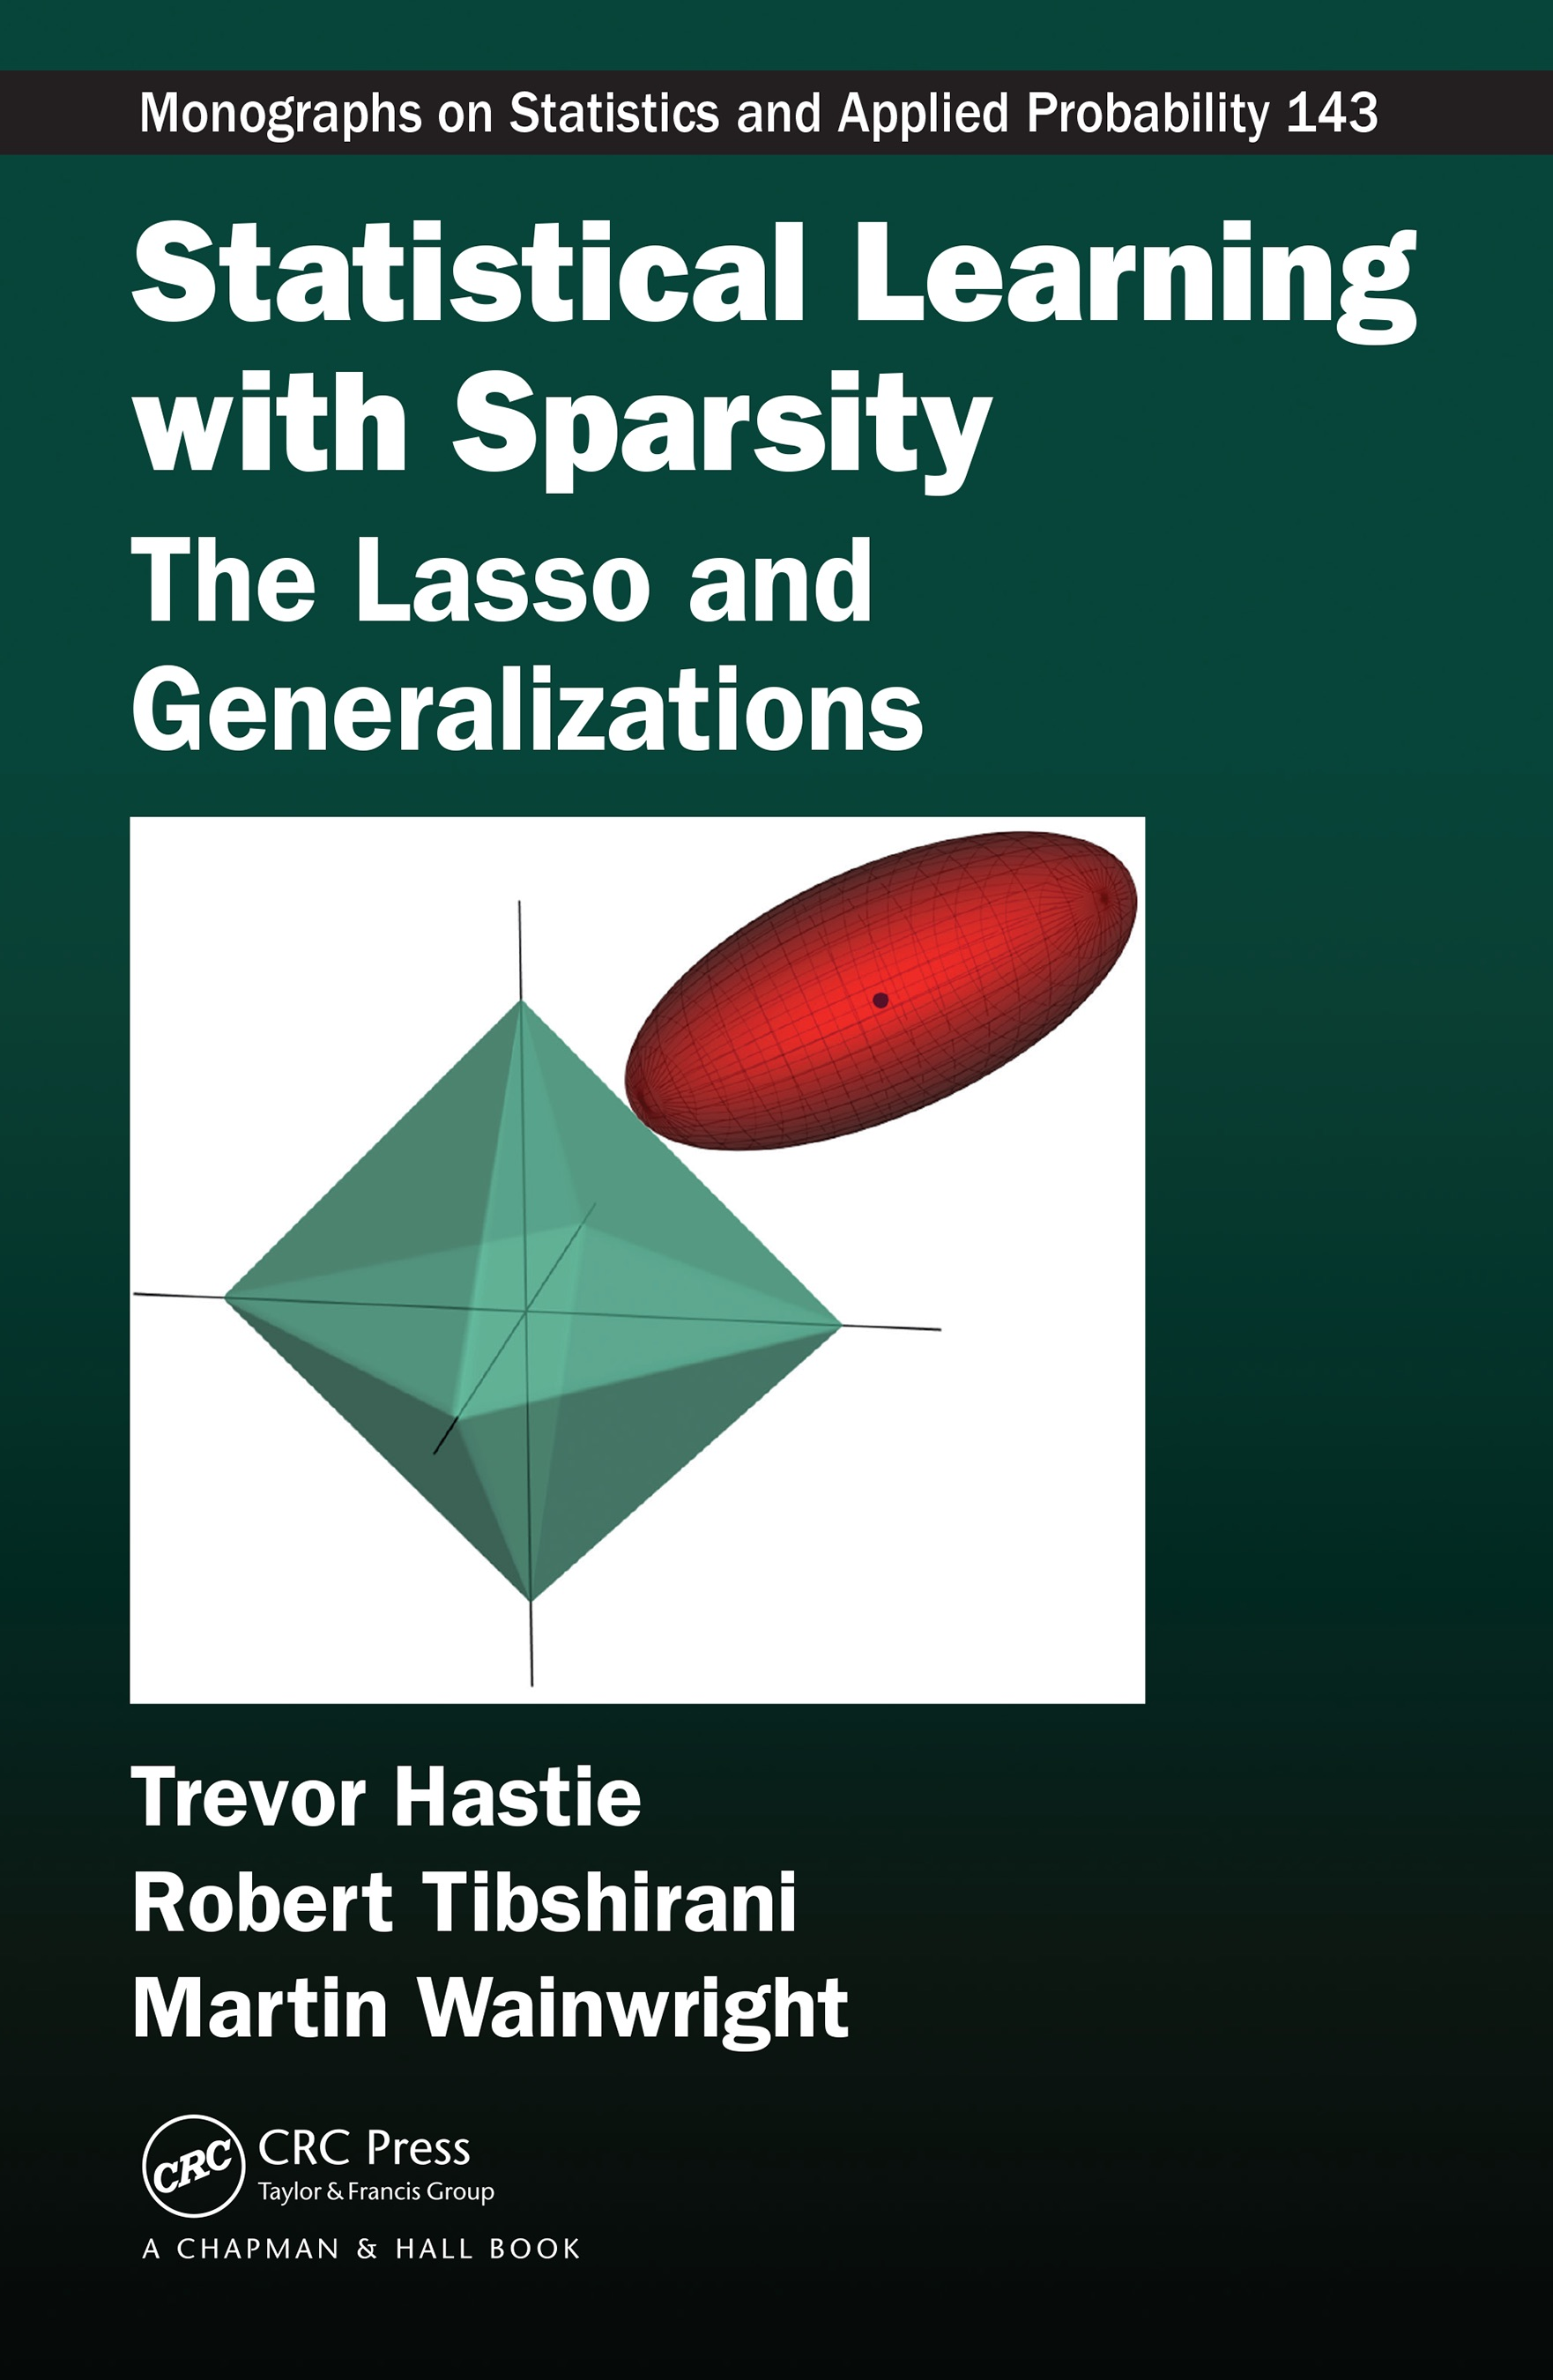
\includegraphics[scale = 0.05]{sls.jpg}
\end{center}
\begin{itemize}
\item \emph{Sparsity} refers to existence of low-dimensional structure hidden in high-dimensional data.\pause
\item E.g. suppose $X$ is 100-dimensional but $Y$ is only a function of $(X_5, X_9)$.\pause
\item Can we exploit sparsity to obtain a good estimate of $I(X; Y)$ even under low sample sizes?
\end{itemize}
\end{frame}

%\begin{frame}
%\frametitle{Dimension reduction vs. sparsity?}
%\begin{columns}
%\begin{column}{0.5\textwidth}
%\begin{center}
%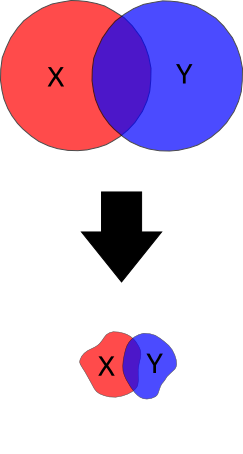
\includegraphics[scale = 0.5]{reduction_unsup.png}
%\end{center}
%Unsupervised dimension reduction
%\pause
%\end{column}
%\begin{column}{0.5\textwidth}
%\begin{center}
%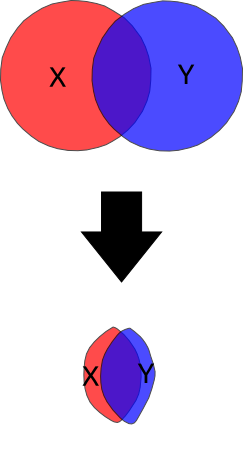
\includegraphics[scale = 0.5]{reduction_sup.png}
%\end{center}
%Sparsity = supervised dim. reduction
%\end{column}
%\end{columns}
%\end{frame}

%\begin{frame}
%\frametitle{Second idea: link prediction accuracy to mutual information}
%\begin{itemize}
%\item If $I(X; Y) > 0$, then $X$ carries information about $Y$ and vice-versa. \pause
%\item Therefore, we can \emph{predict} $Y$ from $X$ (or $X$ from $Y$) \pause
%\item We know that often \emph{prediction accuracy} implies a lower bound for \emph{mutual information} (e.g. %Fano 1952)
%\end{itemize}
%\end{frame}

%\begin{frame}
%\frametitle{Background: Regression}
%\begin{center}
%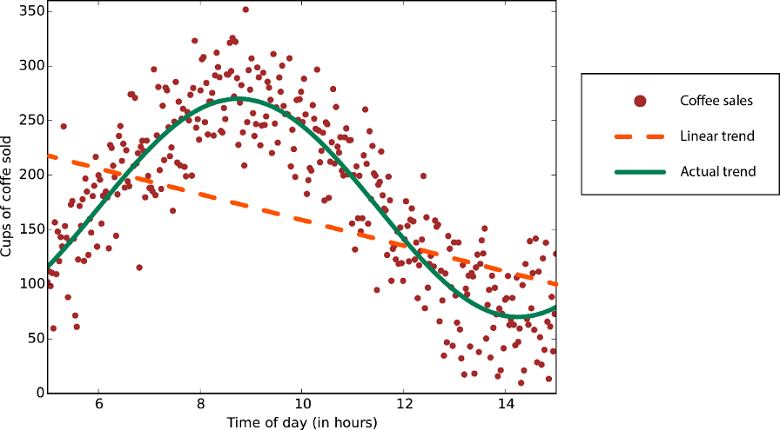
\includegraphics[scale = 0.2]{data_trend.png}
%\end{center}
%\begin{itemize}
%\item Suppose you observe $(\vec{X}^{(i)}, Y^{(i)})_{i=1}^n$ where $Y^{(i)} = f(\vec{X}^{(i)}) + \epsilon$, where $f$ is an unknown function and $\epsilon$ is noise.  (Also, assume $\E[\epsilon] = 0$.)\pause
%\item The goal in regression is to recover the unknown function $f$.\pause
%\item In \emph{linear regression}, we assume $f$ is linear. \pause
%\item if we do not assume a particular form for $f$, we can use \emph{nonparametric regression}.
%\end{itemize}
%\end{frame}

%\begin{frame}
%\frametitle{Background: Sparse regression}
%\begin{itemize}
%\item When $\vec{X}$ is high dimensional, classical regression techniques perform poorly.\pause
%\item If the true function $f$ only depends on a small number of components in $\vec{X}$, we can still do well if %we use \emph{sparse} regression methods.\pause
%\end{itemize}
%\begin{center}
%\begin{tabular}{c|c|c|}
% & \emph{Classical} & \emph{Sparse} \\ \hline
% \emph{Linear} & Ordinary Least-Squares  & Elastic net \\ 
%  & (Legendre 1805) & (Zou 2008)  \\\hline
% \emph{Nonpar.} & LOWESS  & Random forests  \\ 
%   & (Cleveland 1979) & (Breiman 2001)  \\\hline
%\end{tabular}
%\end{center}
%\end{frame}

\begin{frame}
\frametitle{Our proposal}
Suppose we observe pairs $(X_i,Y_i)_{i=1}^n$ iid from density $p(x, y)$.
\begin{enumerate}
\item Estimate a (sparse) regression model for $\E[\vec{Y}|\vec{X}]$.
%\item Estimate the noise model for $Y$.
\item Assess the \emph{prediction accuracy} of the model using \emph{identification loss} (Kay et al. 2008)
\item Use the identification loss to obtain a lower bound for the mutual information $I(X; Y)$
\end{enumerate}
\end{frame}

\begin{frame}
\frametitle{Multiple-response regression}
\begin{itemize}
\item Pairs $(x_i,y_i)_{i=1}^n$, where $X$ is $p$-dimensional and $Y$ is $q$-dimensional.
\item Data matrices $\bX_{n \times p}$, $\bY_{n \times q}$.
\item For each column of $Y$, fit sparse model $Y^{(i)} \approx X^T \beta^{(i)}  + \epsilon$, e.g. by using elastic net (Zou 2008), 
\[
\hat{\beta}^{(i)} = \text{argmin}_\beta ||\bX^T \beta^{(i)} - Y^{(i)}||^2 + \lambda_2 ||\beta^{(i)}||_2^2 + \lambda_1 ||\beta^{(i)}||_1
\]
\item Or, fit a \emph{random forest} model for each column of $Y$ (Breiman 2001)
\end{itemize}
\end{frame}


%\begin{frame}
%\frametitle{Regression vs Identification loss}
%\begin{itemize}
%\item Independent \emph{test set} $(x_i^*, y_i^*)_{i=1}^k$. 
%\item Use model to predict $\hat{y}_i^* = (x_i^*)^T \hat{B}$ for $i = 1,\hdots, k$.
%\end{itemize}
%Two ways to evaluate the predictive accuracy of the regression model:
%\begin{itemize}
%\item Regression (mean squared-error) loss:
%\[
%\text{MSE} = \frac{1}{k} \sum_{i=1}^k ||y_i^* - \hat{y}_i^*||^2.
%\]
%\item Identification loss (Kay 2008):
%\[
%\text{IdLoss}_k = \frac{1}{k} \sum_{i=1}^k (1 - I\{\hat{y}_i^* \text{ is nearest neighbor of }y_i^*\}).
%\]
%\end{itemize}
%\end{frame}

\begin{frame}
\frametitle{Regression vs Identification loss}
\begin{center}
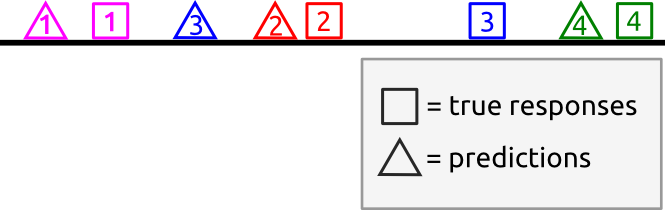
\includegraphics[scale = 0.5]{../diagram/idloss1.png}
\end{center}
\end{frame}

\begin{frame}
\frametitle{Mean-squared error}
\begin{center}
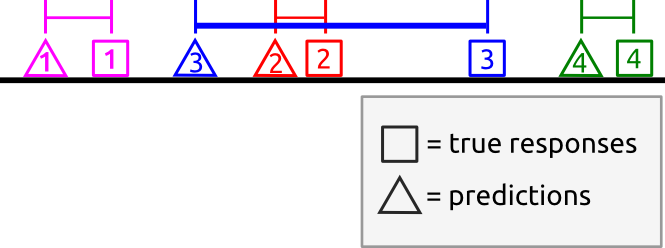
\includegraphics[scale = 0.5]{../diagram/idloss2a.png}
\end{center}
\end{frame}

\begin{frame}
\frametitle{Identification loss}
\begin{center}
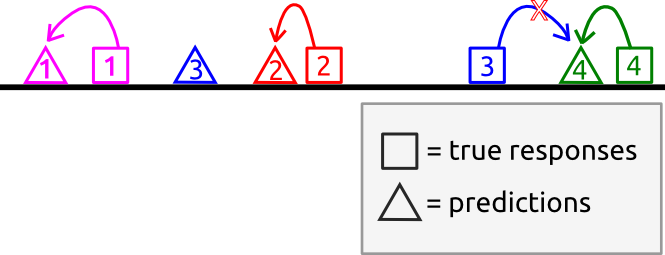
\includegraphics[scale = 0.5]{../diagram/idloss2b.png}
\end{center}
\pause
\begin{itemize}
\item First used by Kay et al. (2008) to compare accuracy of center-surround model of V1 versus Gabor filter model of V1. \pause
\item We are the first to explore theoretical properties of the loss (e.g. connection to mutual information)
\end{itemize}
\end{frame}

%\begin{frame}
%\frametitle{Mean-squared error changes under nonlinear scaling}
%\begin{center}
%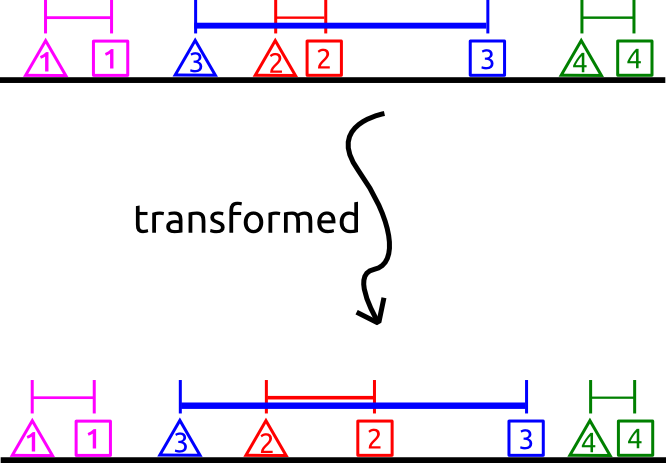
\includegraphics[scale = 0.5]{../diagram/idloss3a.png}
%\end{center}
%\end{frame}

%\begin{frame}
%\frametitle{Identification loss robust under nonlinear scaling}
%\begin{center}
%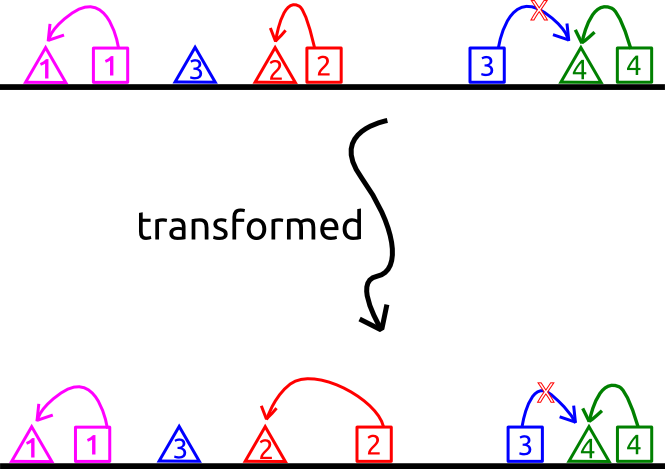
\includegraphics[scale = 0.5]{../diagram/idloss3b.png}
%\end{center}
%\end{frame}


\begin{frame}
\frametitle{Identification loss and mutual information}
\begin{itemize}
\item Define the identification risk as the expected identification loss
\[
\text{IdRisk}_k = \E[\text{IdLoss}_k]
\]
\item \textbf{Theorem.} (Z., Benjamini 2017) There exists a function $g_k$ such that
%For every $k \geq 2$, there exists a function $g_k$ such that
\[I(X; Y) \geq g_k(\text{IdRisk}_k).\]
\end{itemize}
\begin{center}
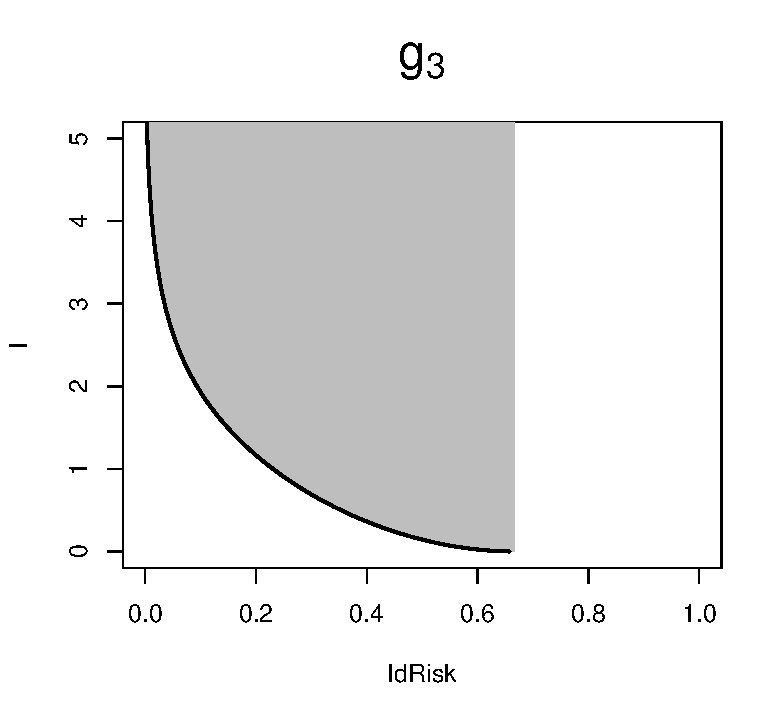
\includegraphics[scale = 0.4]{../idloss/g3.pdf}
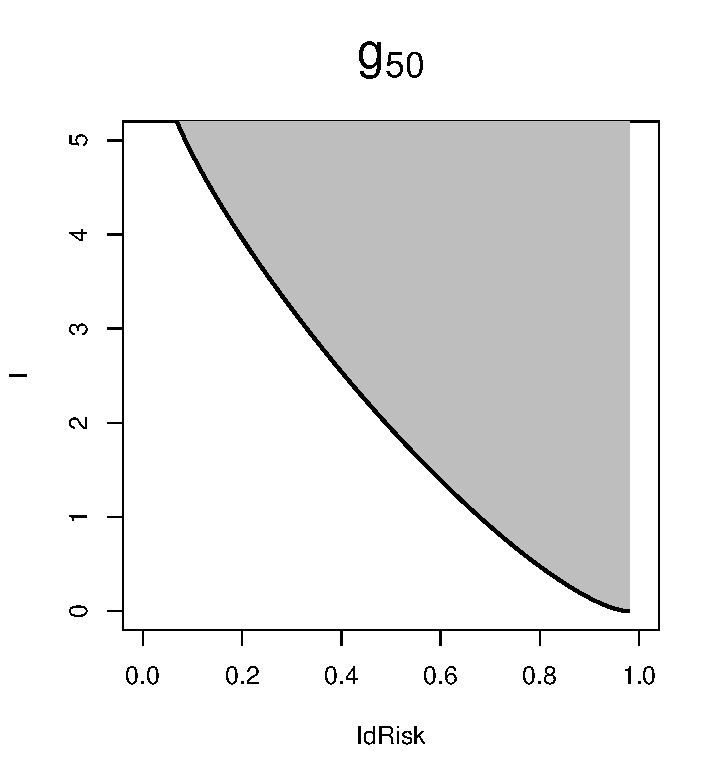
\includegraphics[scale = 0.4]{../idloss/g50.pdf}
\end{center}
\end{frame}


\begin{frame}[label=main]
\frametitle{Proof details}
\begin{columns}
\begin{column}{0.25\textwidth}
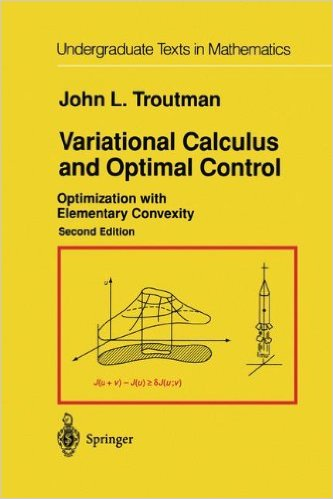
\includegraphics[scale = 0.27]{vcalc.jpg}
\end{column}
\begin{column}{0.75\textwidth}
\begin{itemize}
\item Variational calculus allows optimization of \emph{functionals}.\pause
\item Mutual information is a functional of $p(x, y)$. 
\[
\text{I}[p(x, y)] = \E\left[\log \frac{p(X, Y)}{p(X)p(Y)}\right].
\]
\pause
\item Identification risk is \emph{lower-bounded} by another functional--the \hyperlink{supplemental}{\beamerbutton{Bayes Risk}}. 
\[
\text{BayesRisk}_k[p(x, y)] = 1-\E[\max_{i=1}^k p(Y|X_i)].
\]

\pause
\item $g_k(u)$ obtained by minimizing $\text{I}[p(x, y)]$ subject to $\text{BayesRisk}_k[p(x,y)] \leq u$.
\end{itemize}
\end{column}
\end{columns}
\end{frame}



\begin{frame}
\frametitle{Result}
\textbf{Theorem}.
For any $\iota > 0$, there exists $\beta_\iota \geq 0$ such that defining
\[
q_\beta(t) = \frac{\exp[\beta t^{k-1}]}{\int_0^1 \exp[\beta t^{k-1}]},
\]
we have
\[
\int_0^1 q_{\beta_\iota}(t) \log q_{\beta_\iota}(t) dt = \iota.
\]
Then,
\[
g_k^{-1}(\iota) = \sup_{I(X; Y) = \iota} \text{BayesAcc}_k = \int_0^1 q_{\beta_\iota}(t) t^{k-1} dt.
\]
\end{frame}

\begin{frame}
\frametitle{Our proposal}
Suppose we observe pairs $(X_i,Y_i)_{i=1}^n$ iid from density $p(x, y)$.
\begin{enumerate}
\item Estimate a (sparse) regression model for $\E[\vec{Y}|\vec{X}]$.
\item Compute \emph{identification loss}, $\text{IdLoss}_k$, using \emph{leave-k-out}.
\item Estimate mutual information using
\[
\hat{I}_{IdLoss}(X; Y) = g_k(\text{IdLoss}_k).
\]
\end{enumerate}
\end{frame}

%\begin{frame}
%\frametitle{What is leave-k-out cross-validation?}
%\begin{center}
%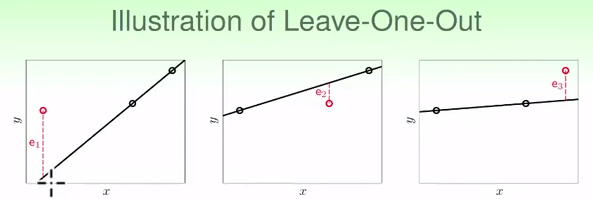
\includegraphics[scale = 0.5]{loocv_sub.png}
%\end{center}
%\begin{itemize}
%\item Randomly hold out a subset of size $k$.
%\item Use remaining data to predict the held-out data.
%\item Obtain the average prediction error.
%\end{itemize}

%{\tiny Image credit Hsuan-Tien Lin}
%\end{frame}

%\item Resulting estimator:
%\[
%\hat{I}_{IdLoss}(X; Y) = g_k(\text{IdLoss}_k).
%\]
%%\item \emph{Remark.} Although $\text{IdLoss}_k$ is unbiased for $\text{IdRisk}_k$, $g_k$ is nonlinear so $\hat{I}_{IdLoss}$ may be biased.



%\begin{frame}
%\frametitle{Cross-validated loss}
%Leave-$k$-out cross-validation (L$k$oCV) can be used for both squared-error loss and identification loss.
%\begin{itemize}
%\item Start with a dataset $(x_i,y_i)_{i=1}^N$.
%\item Let $n = N-k$.  Consider all ${N}\choose{k}$ partitions of the dataset into a test set $(\bX, \bY)$ and training set $(\bX^*, \bY^*)$.
%\item For each partition, compute the loss.
%\item Define the L$k$oCV loss as the average loss over ${N}\choose{k}$ partitions.
%\end{itemize}
%\emph{Computational note}.  One can subsample to avoid computing all
%${N}\choose{k}$ partitions.  In particular, if $m = N/k$, then one can
%use $m$-fold cross-validation which uses $m$ partitions that have
%disjoint test sets.
%\end{frame}




\section{Applications}

\begin{frame}
\sectionpage
\end{frame}

\begin{frame}
\frametitle{Simulation}

%\begin{center}
%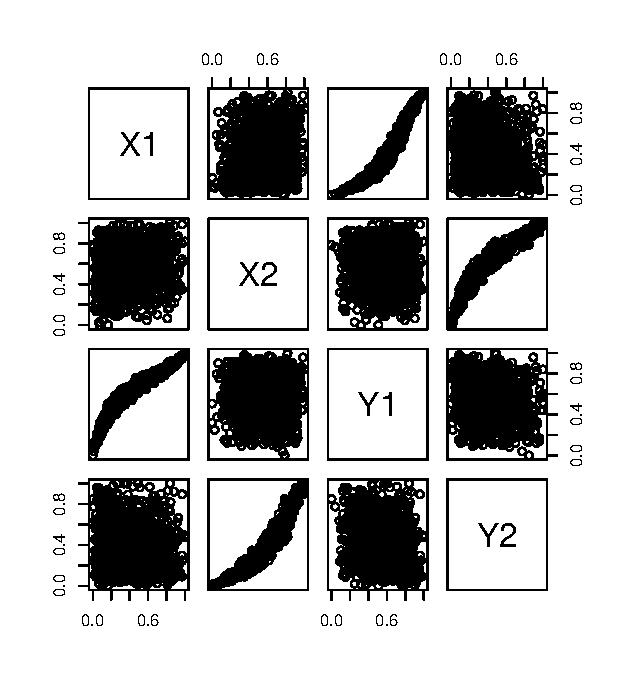
\includegraphics[scale = 0.34]{../idloss/sim1_pairs.pdf}
%\end{center}
\begin{itemize}
\item Generate data: $(Y_1, Y_2) = (X_1, X_2)^T B + \epsilon$\\ where $B$ is a randomly generated coefficient matrix.
\item Add extra noise dimensions $X_3, X_4, \hdots$.
\item $n = 1000$.
\item Compare Nearest-Neighbor estimator (Mnatsakov et al, 2008, implemented in {\tt FNN}) with our method using OLS and elastic net (sparse).
\end{itemize}

\end{frame}

\begin{frame}
\frametitle{Simulation Results - I. low dimension}
\begin{center}
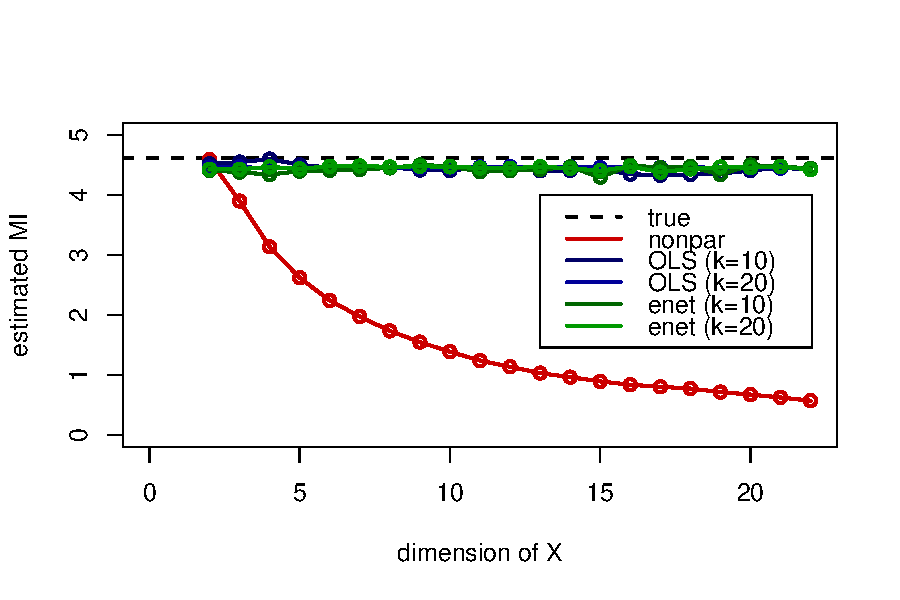
\includegraphics[scale = 0.65]{../idloss/sim2a_fig1.pdf}
\end{center}
\end{frame}

%\begin{frame}
%\frametitle{Simulation Results - I. low dimension}
%\begin{center}
%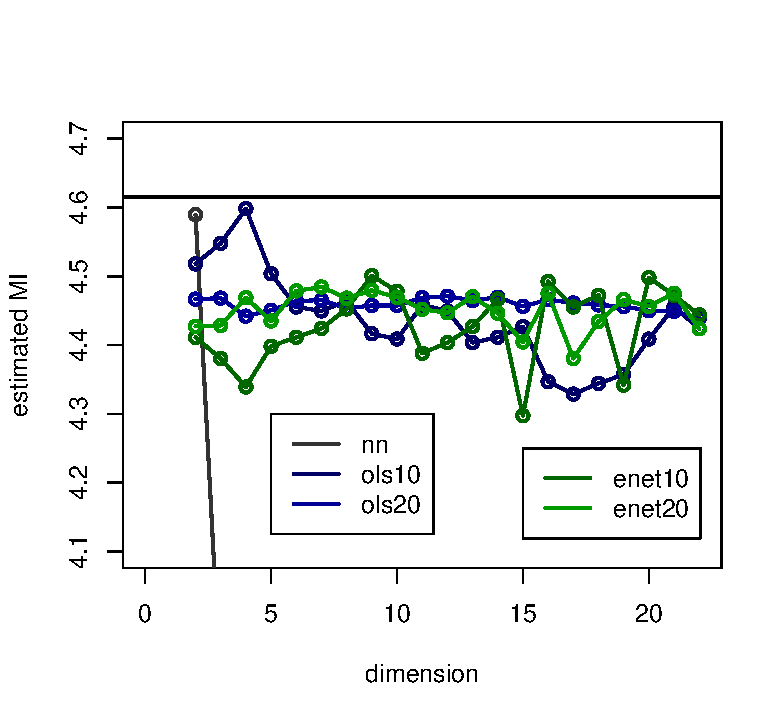
\includegraphics[scale = 0.65]{../idloss/sim2a_fig1a.pdf}
%\end{center}
%\end{frame}

%\begin{frame}
%\frametitle{Simulation Results - II. medium dimension}
%\begin{center}
%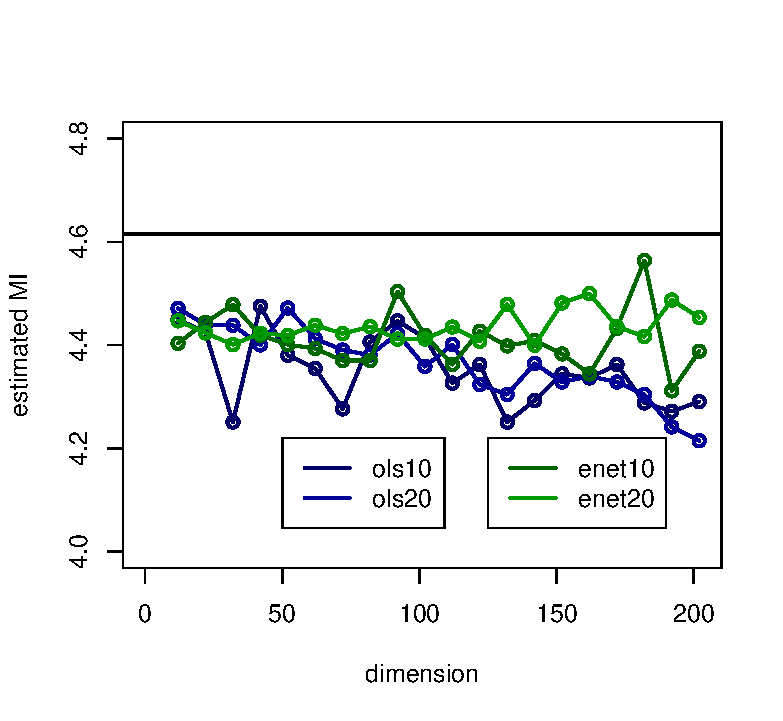
\includegraphics[scale = 0.65]{../idloss/sim2a_fig2.pdf}
%\end{center}
%\end{frame}

\begin{frame}
\frametitle{Simulation Results - III. high dimension}
\begin{center}
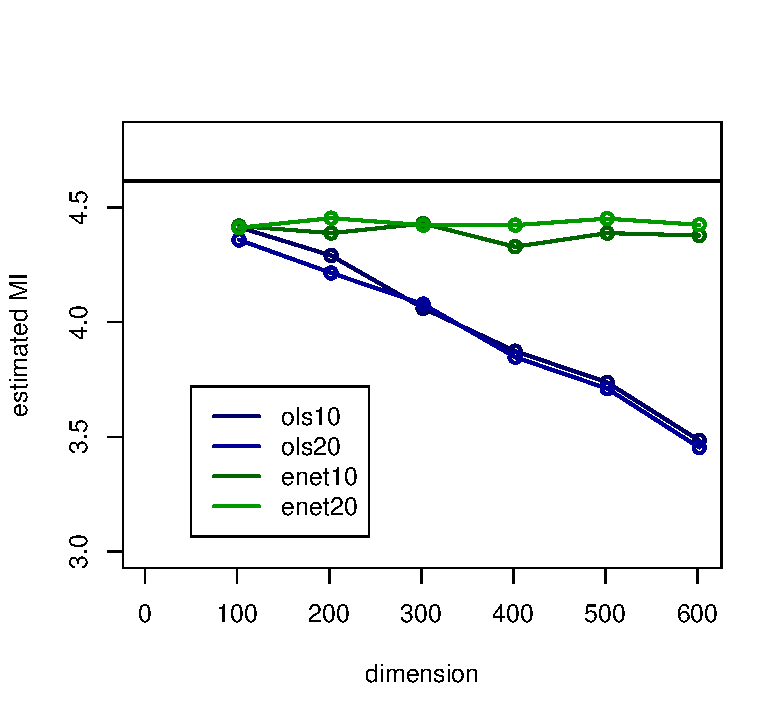
\includegraphics[scale = 0.65]{../idloss/sim2a_fig3.pdf}
\end{center}
\end{frame}






\begin{frame}
\frametitle{Application to gene expression time series}
\begin{columns}
\begin{column}{0.4\textwidth}
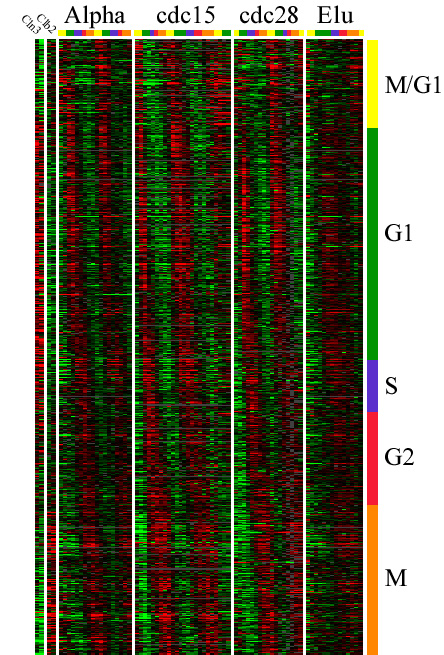
\includegraphics[scale = 0.27]{yeast_cc_fig1.jpg}
\end{column}
\begin{column}{0.6\textwidth}

\begin{itemize}
\item Data from Spellman et al. 1998
\item Expression levels of 6178 yeast genes during cell cycle
\item Total 73 measurements per gene
\end{itemize}
\end{column}
\end{columns}
\end{frame}

\begin{frame}
\frametitle{Groups of genes}
\begin{center}
\begin{tabular}{c|c}
Group & No. genes \\ \hline
unknown & 396 \\
cell cycle & 27 \\
DNA replication & 27 \\
transport & 19 \\
cytoskeleton & 17\\
chromatin structure & 16 \\\hline
\end{tabular}
\end{center}

\vspace{0.5in}
Total 145 different categories (only top 6 shown).
\end{frame}

%# [,1] [,2] [,3]      [,4]      [,5]
%# [1,]    0    1    1 1.0000000 1.0000000
%# [2,]    0    0    1 0.9988279 0.9994315
%# [3,]    0    0    0 0.9911839 0.9897579
%# [4,]    0    0    0 0.0000000 0.9891288
%# [5,]    0    0    0 0.0000000 0.0000000

\begin{frame}
\frametitle{Canonical correlations between time series}
Top canonical correlation (Hotelling 1936)

\begin{center}
\begin{tabular}{c|c|c|c|c|c|} 
   & CC   & DR   & Tr   & Cy   & CS  \\ \hline
CC &      & 1    & 1    & 1    & 1   \\ \hline
DR &      &      & 1    & 0.99 & 0.99\\ \hline
Tr &      &      &      & 0.99 & 0.98\\ \hline
Cy &      &      &      &      & 0.98\\ \hline
CS &      &      &      &      &     \\ \hline
\end{tabular}
\end{center}

\vspace{0.5in}
CC = cell cycle, DR = DNA replication, Tr = transport, \\
Cy = cytoskeleton, CS = chromatin structure
\end{frame}


%# [,1]      [,2]      [,3]      [,4]      [,5]
%# [1,]    0 0.9570214 0.8734071 0.9245117 0.9358656
%# [2,]    0 0.0000000 0.8325764 0.8856461 0.9500084
%# [3,]    0 0.0000000 0.0000000 0.8329383 0.7832109
%# [4,]    0 0.0000000 0.0000000 0.0000000 0.9001239
%# [5,]    0 0.0000000 0.0000000 0.0000000 0.0000000

\begin{frame}
\frametitle{Sparse canonical correlations between time series}
Using sparse CCA* (Witten and Tibshirani 2009).

\begin{center}
\begin{tabular}{c|c|c|c|c|c|} 
   & CC   & DR   & Tr   & Cy   & CS \\ \hline
CC &      & 0.96 & 0.87 & 0.92 & 0.94\\ \hline
DR &      &      & 0.83 & 0.88 & 0.95\\ \hline
Tr &      &      &      & 0.83 & 0.78\\ \hline
Cy &      &      &      &      & 0.90\\ \hline
CS &      &      &      &      &     \\ \hline
\end{tabular}
\end{center}

\vspace{0.5in}
CC = cell cycle, DR = DNA replication, Tr = transport, \\
Cy = cytoskeleton, CS = chromatin structure

\vspace{0.1in}

\tiny{*: using {\tt CCApermute} in R package {\tt PMA}}
\end{frame}


%# [,1]      [,2]      [,3]      [,4]      [,5]
%# [1,] 0.0000000 0.9288215 0.7770040 0.9767242 0.8293687
%# [2,] 0.9288215 0.0000000 0.8496598 0.9102823 0.9200308
%# [3,] 0.7770040 0.8496598 0.0000000 0.7165050 0.7147406
%# [4,] 0.9767242 0.9102823 0.7165050 0.0000000 0.9303434
%# [5,] 0.8293687 0.9200308 0.7147406 0.9303434 0.0000000

\begin{frame}
\frametitle{Information correlations between time series}
Taking the max of $\hat{I}(X; Y)$ and $\hat{I}(Y; X)$.

\begin{center}
\begin{tabular}{c|c|c|c|c|c|} 
   & CC   & DR   & Tr   & Cy   & CS \\ \hline
CC &      & 0.93 & 0.78 & 0.98 & 0.83\\ \hline
DR &      &      & 0.85 & 0.91 & 0.92\\ \hline
Tr &      &      &      & 0.72 & 0.71\\ \hline
Cy &      &      &      &      & 0.93\\ \hline
CS &      &      &      &      &     \\ \hline
\end{tabular}
\end{center}

\vspace{0.5in}
CC = cell cycle, DR = DNA replication, Tr = transport, \\
Cy = cytoskeleton, CS = chromatin structure
\end{frame}

%\begin{frame}
%\frametitle{Comparing sparse CCA and $Cor_{Info}$}
%\begin{center}
%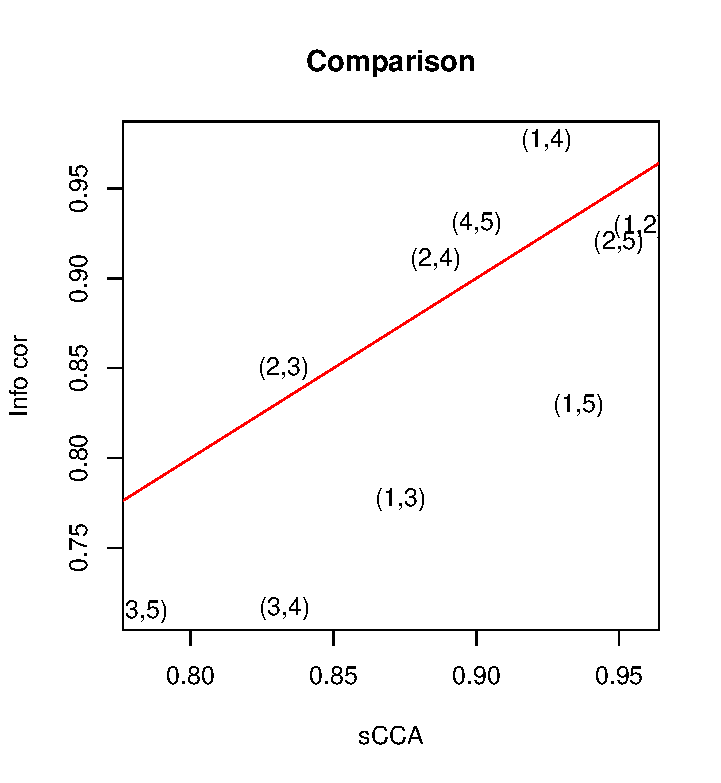
\includegraphics[scale = 0.5]{../idloss/cca_p_vs_info_cor.pdf}
%\end{center}
%(1) cell cycle, (2) DNA replication, (3) transport, \\
%(4) cytoskeleton, (5) chromatin structure
%\end{frame}

\begin{frame}
\frametitle{Invariance properties}
\begin{itemize}
\item Transform data from each group with random rotation...
\[\tilde{bX} = \bX E\]
\[\tilde{bY} = \bX F\]
with $E^T E = I$, $F^T F = I$.\pause
\item CCA is invariant:
\[
\text{CCA}(\bX, \bY) = \text{CCA}(\tilde{bX},\tilde{bY})
\]
\pause
\end{itemize}
\end{frame}

\begin{frame}
\frametitle{Invariance properties}
However, sparse CCA is not invariant.

\begin{center}
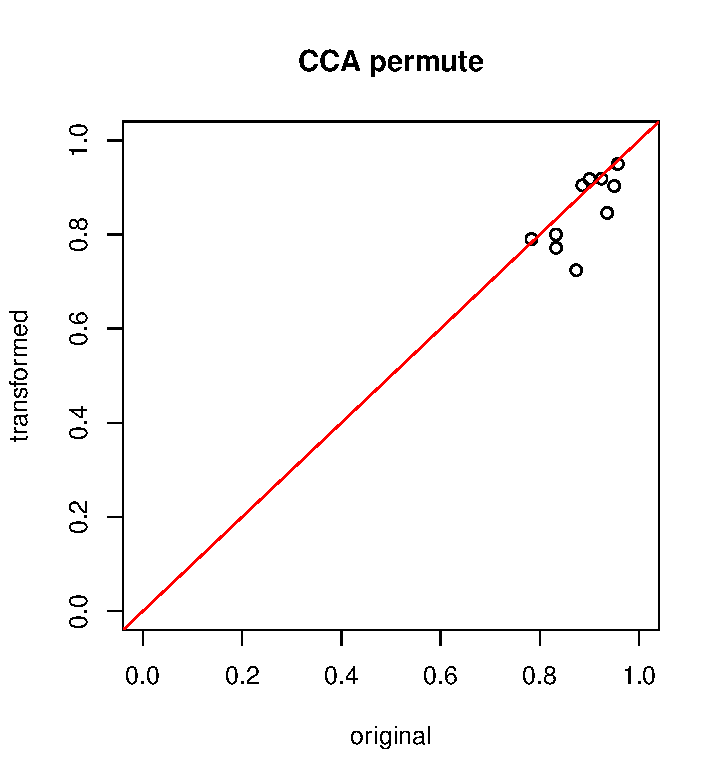
\includegraphics[scale = 0.5]{../idloss/cca_p_robustness.pdf}
\end{center}
\end{frame}

\begin{frame}
\frametitle{Invariance properties}
Our method, on the other hand, is \emph{robust} to rotation.

\begin{center}
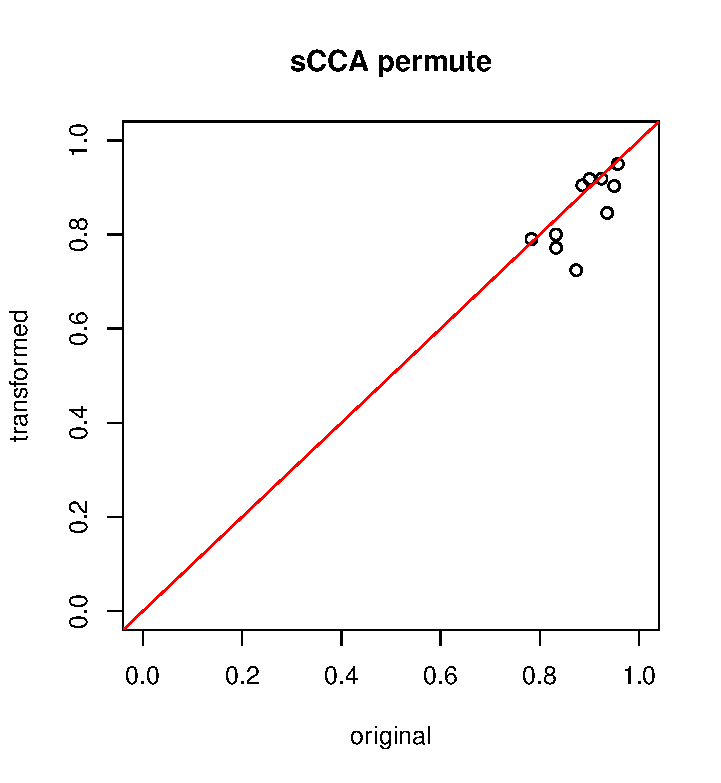
\includegraphics[scale = 0.5]{../idloss/info_cor_robustness.pdf}
\end{center}
\end{frame}

\begin{frame}
\frametitle{Conclusions}
\begin{itemize}
\item Mutual information, and derived $\text{Cor}_{Info}$ are useful measures of correlation, but hard to estimate.\pause
\item Our method targets high-dimensional data with sparsity.\pause
\item How to use: choose a regression model suited to the model
  assumptions.  Our method allows you to convert the prediction
  accuracy of the model, $\text{IdLoss}_k$ into an estimate of $I(\vec{X};
  \vec{Y})$.\pause
\item Example application: measure of joint information between two tables which is robust to transformations.
\end{itemize}
\end{frame}

\begin{frame}
\frametitle{Related work and future directions}
\begin{itemize}
\item What if data is high-dimensional, but not sparse?  We have another method based on high-dimensional asymptotics (ZB 2016).\pause
\item Estimating quantities related to mutual information, such as \emph{transfer information}, \emph{stimulus-specific information} and \emph{redundancy} (Borst and Theunissen 1999) \pause
\item Inferring resting-state brain networks.
\begin{center}
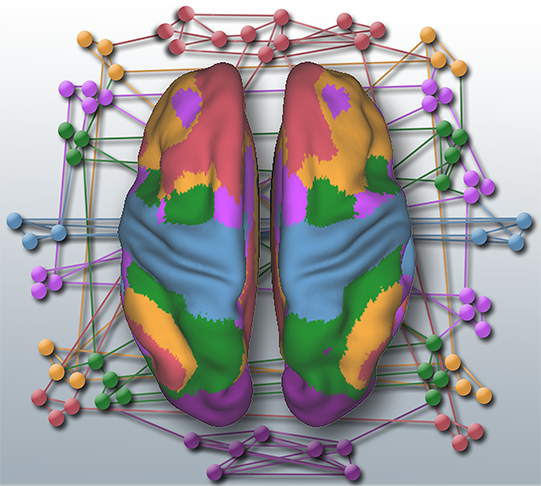
\includegraphics[scale = 0.5]{cmsIMG_6589b1.png}
\end{center}
{\tiny Image credit Simons Foundation}
\end{itemize}
\end{frame}

\section{The End}

\begin{frame}
\sectionpage
\end{frame}

\begin{frame}
\frametitle{References}
{\tiny
\begin{itemize}
\item Reshef et al, 2011. ``Detecting Novel Associations in Large Datasets.'' \emph{Science}.
\item Speed, 2011. ``A correlation for the 21st century.'' \emph{Science}.
\item Linfoot, 1957.  ``An informational measure of correlation.''  \emph{Information and Control}.
\item Kay, 2008.  ``Identifying natural images from human brain activity.''  \emph{Nature}.
\item Mnatsakanov, et al, (2008). ``K-nearest neighbor estimators of entropy.'' \emph{Mathematical Methods of Statistics}
\item Spellman et al., (1998).  ``Comprehensive Identification of Cell Cycle-regulated Genes of the Yeast Saccharomyces cerevisiae by Microarray Hybridization.''  \emph{Molecular Biology of the Cell}. 
\item Hotelling, H. (1936). ``Relations Between Two Sets of Variates''. \emph{Biometrika.}
\item Witten, Daniela M., and Robert J. Tibshirani. (2009). ``Extensions of sparse canonical correlation analysis with applications to genomic data.'' \emph{Statistical applications in genetics and molecular biology}
\end{itemize}
}
\end{frame}


\begin{frame}[label=supplemental]
\frametitle{Intuition behind identity}
\[
\text{BayesRisk}_k[p(x, y)] = 1 - \text{BA}_k[p(x, y)] = 1-\E[\max_{i=1}^k p(Y|X_i)].
\]
\begin{columns}
\begin{column}{0.5\textwidth}
\begin{center}
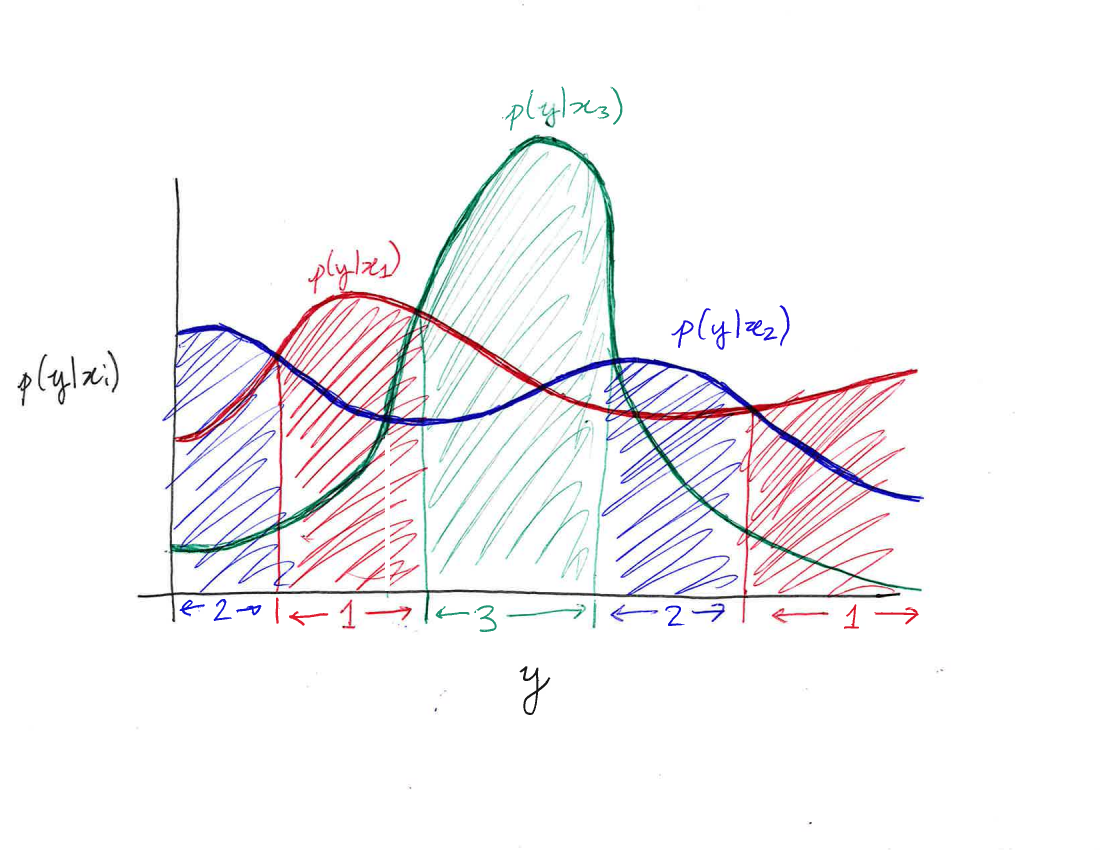
\includegraphics[scale = 0.35, clip = true, trim = 1.2in 1.3in 0in 1in]{var_ba.png}
\end{center}   
\end{column}
\begin{column}{0.5\textwidth}  %%<--- here
\begin{align*}
\text{BA}&(x_1,x_2,x_3) \\&= \sum_i \Pr[x_i]\Pr_{Y \sim p(y|x_i)}[Y \in \text{zone }i]
\\&= \sum_i \frac{1}{k} \text{Area under curve $i$ in zone $i$}
\\&\ \ \ = \frac{1}{k} \text{Area under } \max_{i=1}^k p(y|x_i)
\end{align*}
\end{column}
\end{columns}
Back to \hyperlink{main}{\beamerbutton{main}}.
\end{frame}

\end{document}

\begin{frame}
\frametitle{Reduced Problem}
Rather than show the whole proof, we consider a simplified problem to illustrate the methods.
\begin{center}
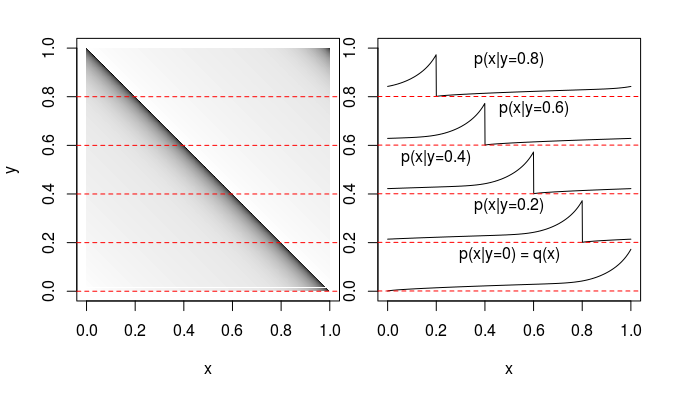
\includegraphics[scale = 0.5]{../diagram/qxplot.png}
\end{center}

Actually, the simplified problem is equivalent to the full problem and we get the same answer (but this is non-trivial).
\end{frame}

\begin{frame}
\frametitle{Reduced Problem}

\begin{center}
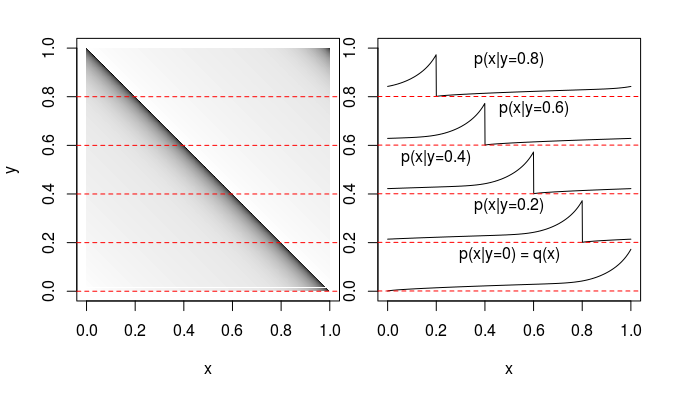
\includegraphics[scale = 0.4]{../diagram/qxplot.png}
\end{center}

\begin{itemize}
\item $p(x, y)$ on unit square with uniform marginals.
\item The conditional distributions $p(x|y)$ are just ``shifted'' copies of a common density, $q(x)$, on $[0,1]$
\[
p(x|y) = q(x - y + I\{x < y\})
\]
\item Furthermore, $q(x)$ is increasing in $x$.
\end{itemize}

\end{frame}

\begin{frame}
\frametitle{Simplified formulae}

The information and average Bayes error can be written in terms of $q(x)$.

\[
\text{I}[p(x, y)] = \int_0^1 q(x) \log q(x) dx
\]
\[
\text{BayesAcc}_k[p(x, y)] = \int_{[0, 1]^k} \max_{i=1}^k q(x_i) dx_1 \cdots dx_k
\]



\end{frame}

\begin{frame}
\frametitle{Simplified formulae}

Overload the notation and ``redefine'' information and average Bayes error as functionals of $q(x)$.

\[
\text{I}[q(x)] \stackrel{def}{=} \int_0^1 q(x) \log q(x) dx
\]
\[
\text{BayesAcc}_k[q(x)] \stackrel{def}{=} \frac{1}{k}\int_{[0, 1]^k} \max_{i=1}^k q(x_i) dx_1 \cdots dx_k
\]

\end{frame}

\begin{frame}
\frametitle{Optimization problem}
We now pose the question: how do we find $q(x)$ which maximizes $\text{BayesAcc}_k[q(x)]$ subject to $\text{I}[q(x)] \leq \iota$?

\begin{itemize}
\item \emph{Domain of the optimization}: Recall that $q(x)$ satisfies $q(x) \geq 0$, $\int_0^1 q(x) dx = 1$, and is increasing in $x$.
Let $\mathcal{Q}$ denote the space of functions on $[0,1] \to [0,\infty)$ which are increasing in $x$.
\item \emph{Constraints}: We have two remaining constraints, $\text{I}[q(x)] \leq \iota$ and $\int_0^1 q(x) dx = 1$.
\end{itemize}

Hence the problem is
\[
\text{maximize}_{q(x) \in \mathcal{Q}}\text{ BayesAcc}_k[q(x)]\text{ subject to }\int_0^1 q(x) dx = 1\text{ and }\text{I}[q(x)] \leq \iota.
\]
\end{frame}


\begin{frame}
\frametitle{Optimization problem}
\[
\text{maximize}_{q(x) \in \mathcal{Q}}\text{ BayesAcc}_k[q(x)]\text{ subject to }\int_0^1 q(x) dx = 1\text{ and }\text{I}[q(x)] \leq \iota.
\]
\begin{itemize}
\item Does a solution exist? \emph{Yes}, because the space of measures
  with density $q(x)$ satisfying $\text{I}[q(x)] \leq \iota$ is tight,
  and both the constraints and objective are continuous wrt to the
  topology of weak convergence.
\item Given a solution $q^*(x)$ exists, there exist Lagrange multipliers $\lambda \in \mathbb{R}$ and $\nu > 0$ such that $q^*$ minimizes
\begin{align*}
\mathcal{L}[q(x)] &= -\text{BayesAcc}_k[q(x)] + \lambda \int_0^1 q(x) dx + \nu \text{I}[q(x)]
\\&= \int_0^1 (-t^{k-1} + \lambda + \nu \log q(x)) q(x) dx.
\end{align*}
\end{itemize}

\end{frame}

\begin{frame}
\frametitle{Functional derivatives}
\begin{itemize}
\item Taylor explansions are a useful trick for computing functional derivatives
\item We can compute the functional derivative of $\mathcal{L}[q(x)]$ by writing
\begin{align*}
\mathcal{L}[q(x) + \epsilon \xi(x)] &
\\= \int_0^1 (-t^{k-1} &+ \lambda + \nu \log (q(x) + \epsilon \xi(x))) (q(x) + \epsilon \xi(x)) dx.
\\\approx  \int (q(x) + &\epsilon \xi(x)) (-t^{k-1} + \lambda + \nu \{\log q(x) + \frac{\epsilon \xi(x)}{q(x)}\}) dx
\\\approx  \mathcal{L}[q(x)] +& \int_0^1 (-t^{k-1} + \lambda + \nu (1 + \log q(x)) \epsilon\xi(x) dx.
\end{align*}
\item Hence
\[
\nabla \mathcal{L}[q](x) = -t^{k-1} + \lambda + \nu (1 + \log q(x))
\]
\end{itemize}
\end{frame}

\begin{frame}
\frametitle{Variational magic!}
Suppose we set the functional derivative to 0,
\[
0 = \nabla \mathcal{L}[q](t) = -t^{k-1} + \lambda + \nu + \nu \log q(t).
\]
Then we conclude that the optimal $q^*(t)$ takes the form
\[
q^*(t) = \alpha e^{\beta t^{k-1}}
\]
for some $\alpha > 0$, $\beta > 0$.

From the constraint $\int q(t)dt = 1$, we get
\[
q_\beta(t) = \frac{e^{\beta t^{k-1}}}{\int e^{\beta t^{k-1}} dt}.
\]
\end{frame}










\end{document}
